\section{Methodische Vorgehensweise}
\subsection{Datenerhebung}
Für die Gegenüberstellung der Technologietrends in der akademischen Forschung und praktizierenden Wirtschaft werden, wie bereits in Abschnitt \ref{sec:method} erwähnt, zwei Arten von Quellen herangezogen.
\subsubsection{Gartner Hype Cycle for Emerging Technologies}

Der \glqq Gartner Hype Cycle for Emerging Technologies\grqq~repräsentiert als markt\-führendes Beratungsunternehmen für Technologieprognosen den Part der praktizierenden Wirtschaft. Dabei dienen die Technologien im Bereich der \glqq Peak of Inflated Expectations\grqq~in vorliegender Reihenfolge als Datenbasis für die Analyse, da sie den Höhepunkt der Trendwahrnehmung darstellen.

Für die optimale Ausrichtung der Analyse an die Leitfragen ist es sinnvoll, eine relativ aktuelle Ausgabe des \glqq Hype Cycle\grqq~zu verwenden, nicht jedoch die neuste. Denn für die Leitfrage L3 wird mindestens eine neuere Ausgabe als die analysierte benötigt. Bei zu alten Publikationen besteht wiederum die Gefahr, dass durch gegenseitige Einflussnahme eine Angleichung bspw. der Begrifflichkeiten die Ergebnisse verfälschen könnte.

Die aktuellste Ausgabe des \glqq Gartner Hype Cycle for Emerging Technologies\grqq~ ist im Juli 2017 erschienen.\footnote{\citeNP<Vgl.>[o.S.]{ghc2017}} Deshalb fällt die Wahl auf die unmittelbar vorausgegangene Veröffentlichung aus dem Jahre 2016. Im Abschnitt \glqq Peak of Inflated Expectations\grqq~sind folgende Technologien aufgeführt:\footnote{\citeNP<Vgl.>[o.S.]{ghc2016}}

\begin{itemize}
	\item Gesture Control Devices
	\item Micro Data Centers
	\item Smart Robots
	\item Blockchain
	\item Connected Home
	\item Cognitive Expert Advisors
	\item Machine Learning
	\item Software-Defined Security
	\item Autonomous Vehicles
	\item Nanotube Electronics
	\item Software-Defined Anything (SDx)
\end{itemize}

In Abbildung \ref{fig:ghc2016} ist der dazugehörige Graph zu sehen, dem zusätzlich die Erwartungen an die Technologie in Abhängigkeit zum Reifegrad sowie die voraussichtliche Dauer bis zur Erreichung des \glqq Plateau of Productivity\grqq~entnommen werden können.

\begin{figure}
	\centering
	\caption{Gartner Hype Cycle for Emerging Technologies, 2016}
	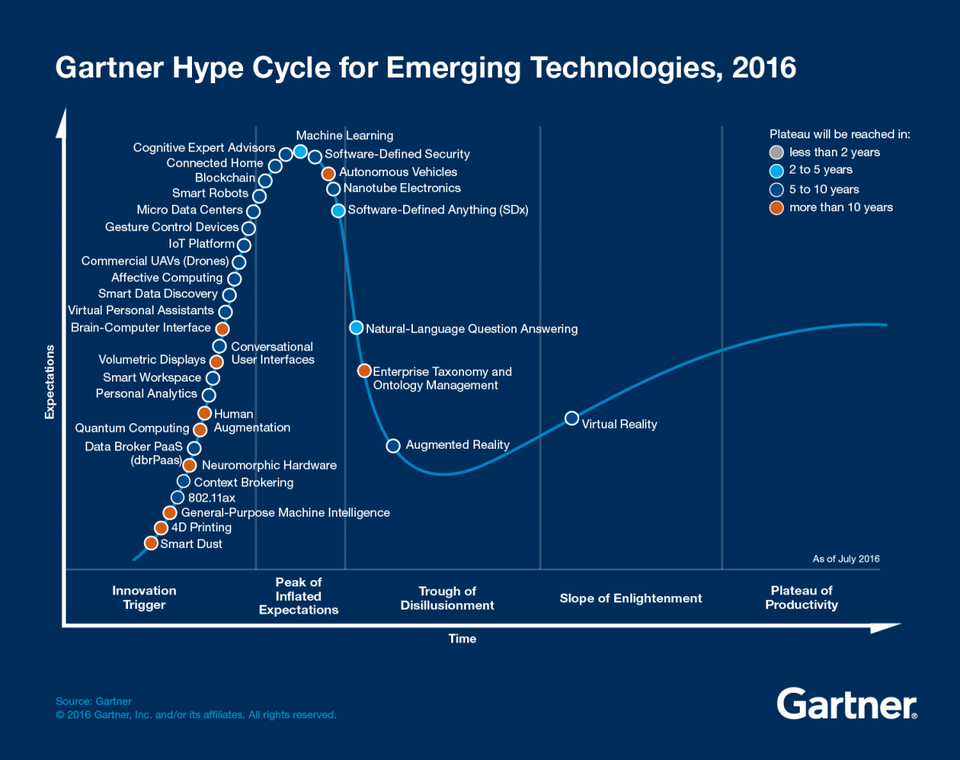
\includegraphics[width=0.9\linewidth]{img/Hype_Cycle_2016.jpg}
	\caption*{\protect\citeNP<Quelle:>[o.S.]{ghcet2016}}
	\label{fig:ghc2016}
\end{figure}

Demnach sind die Erwartungen und somit die Trendwahrnehmung für die Technologie \glqq Machine Learning\grqq~am höchsten. Die Technologien links davon haben eine geringere Reife, die rechts davon eine höhere. Insgesamt handelt es sich bei den Technologien allesamt um Trends des Jahres 2016 in der praktizierenden Wirtschaft.

Um den Trendverlauf der ausgewählten Technologien zu bestimmen, müssen weitere \glqq Hype Cyles\grqq~betrachtet werden. Das erstmalige Erscheinen in einer Publikation liefert einen Hinweis darauf, wann eine Technologie die Aufmerksamkeit der relevanten Gruppe von praktizierenden Wirtschaftlern erlangt hat.

Zur Ermittlung des erstmaligen Erscheinens werden diese zunächst einmal in vergangenen Publikationen gesucht.







\subsubsection{Literaturdatenbanken}
Demgegenüber wird die Datenbasis der akademischen Forschung aus Abfragen in relevanten Literaturdatenbanken erhoben. Aufgrund ihrer hohen Abdeckung wissenschaftlich, technologischer Publikationen werden folgende Datenbanken durchsucht:
\begin{itemize}
	\item Web of Science Core Collection: \url{http://apps.webofknowledge.com}
	\item IEEE Xplore Digital Library: \url{https://ieeexplore.ieee.org}
	\item The ACM Guide to Computing Literature: \url{https://dl.acm.org}
\end{itemize}

\subsection{Operationalisierung der Daten}
Verstehen der Technologien
Synonyme finden
unterschiedliche Begrifflichkeiten feststellen
Kurve über die Zeit in Abhängigkeit zu Erwartungen

\subsection{Methodik der Analyse}